% \documentclass[handout]{beamer}
\documentclass{beamer}

\usetheme[progressbar=frametitle]{metropolis}
\usepackage{appendixnumberbeamer}
\usepackage{booktabs}
\usepackage{amsmath}
\usepackage{comment}

\usepackage{amssymb}
\usepackage{tcolorbox}
\usepackage{tikz}
\usetikzlibrary{bayesnet}
\definecolor{metropolisblue}{RGB}{39, 59, 94}

% Define custom colors
\definecolor{myblue}{HTML}{007AFF}
\definecolor{mygreen}{HTML}{4CD964}
\definecolor{myred}{HTML}{FF3B30}
\definecolor{myorange}{HTML}{FF9500}

% Begin document
\begin{document}

% Title page
\title{Maximum A Posteriori Estimation}
\author{Nipun Batra}
\date{\today}
\institute{IIT Gandhinagar}
\maketitle
\setbeamercovered{invisible}
\begin{frame}
    \frametitle{Agenda}
    \tableofcontents[hidesubsections]
    \end{frame}

\begin{section}{Revision}
    \begin{frame}{Bayes Rule}
        \begin{equation*}
            \textcolor{myblue}{P(\theta|D)} = \frac{\textcolor{mygreen}{P(D|\theta)} \cdot \textcolor{myred}{P(\theta)}}{\textcolor{myorange}{P(D)}}
        \end{equation*}
        
        \begin{itemize}
            \item \textcolor{myblue}{$P(\theta|D)$} is called the posterior
            \item \textcolor{mygreen}{$P(D|\theta)$} is called the likelihood
            \item \textcolor{myred}{$P(\theta)$} is called the prior
            \item \textcolor{myorange}{$P(D)$} is called the evidence
        \end{itemize}
    \end{frame}

    \begin{frame}{Maximum Likelihood Estimation}
        \begin{equation*}
            \textcolor{myblue}{P(\theta|D)} = \frac{\textcolor{mygreen}{P(D|\theta)} \cdot \textcolor{myred}{P(\theta)}}{\textcolor{myorange}{P(D)}} = \frac{\textcolor{mygreen}{P(D|\theta)} \cdot \textcolor{myred}{P(\theta)}}{\int_{\theta} \textcolor{mygreen}{P(D|\theta)} \cdot \textcolor{myred}{P(\theta)} d\theta}
        \end{equation*}
        %tcolorbox
        \begin{tcolorbox}[colback=metropolisblue!5,colframe=metropolisblue,title=]
            Given a dataset $D$, find the parameters $\theta$ that maximize the likelihood of the data.
            \begin{equation*}
                \theta_{\text{MLE}} = \arg \max_{\theta} \textcolor{mygreen}{P(D|\theta)}
            \end{equation*}
        For example, given a linear regression problem setup, we set the likelihood as normal distribution and find the parameters $\theta$ that maximize the likelihood of the data.
        \end{tcolorbox}
    \end{frame}
    
    
    \begin{frame}{Maximum A Posteriori Estimation}
        \begin{equation*}
            \textcolor{myblue}{P(\theta|D)} = \frac{\textcolor{mygreen}{P(D|\theta)} \cdot \textcolor{myred}{P(\theta)}}{\textcolor{myorange}{P(D)}} = \frac{\textcolor{mygreen}{P(D|\theta)} \cdot \textcolor{myred}{P(\theta)}}{\int_{\theta} \textcolor{mygreen}{P(D|\theta)} \cdot \textcolor{myred}{P(\theta)} d\theta}
        \end{equation*}
        %tcolorbox
        \begin{tcolorbox}[colback=metropolisblue!5,colframe=metropolisblue,title=]
            Given a dataset $D$, find the parameters $\theta$ that maximize the posterior of $\theta$ considering both the likelihood and the prior.
            \begin{equation*}
                \theta_{\text{MAP}} = \arg \max_{\theta} \textcolor{myblue}{P(\theta|D)} = \arg \max_{\theta} \textcolor{mygreen}{P(D|\theta)} \cdot \textcolor{myred}{P(\theta)}
            \end{equation*}
        \end{tcolorbox}
    \end{frame}

    \begin{frame}{Maximum A Posteriori Estimation}
        \begin{itemize}
            \item \textbf{MLE}: Given N observations, obtain best $\theta$ estimate (or $\theta_{MLE}$)
            \pause
            % \item Suppose 10 coin tosses observed 4 heads and 6 tails. What is the best estimate of $P(H) = \theta$?
            \item What if we have prior knowledge about $\theta$? %of the coin?
            \pause
            \item \textbf{MAP}: Given N observations and prior knowledge, obtain best $\theta$ estimate (or $\theta_{MAP}$)
            \pause
            \item When do we need prior knowledge?
            \pause  
            \begin{itemize}
                \item When the dataset is not a good representation of the true distribution.
                \item Can be a data quality and/or quantity issue.
            \end{itemize}
        \end{itemize}
    \end{frame}

\end{section}

\begin{section}{Coin Toss Problem}
    \begin{frame}{Coin Toss Problem}
        \begin{itemize}
            \item Consider a sequence of independent N coin toss outcomes, $D = \{ y_1, ... , y_N \}$ where 
            each observation $y_i$ is a binary random variable (Heads: 1, Tails: 0).
            \pause
            \item Assuming $y_i \sim \text{Bernoulli} \left( \theta \right)$, $P (y_i | \theta) = \theta^{y_i} (1 - \theta)^{1 - y_i}$
      
        \end{itemize}
        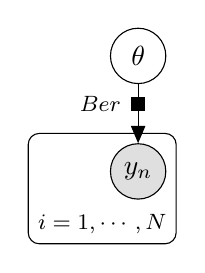
\begin{tikzpicture}
                    
            \node[obs]                               (xn) {$y_n$};
            \factor[above=of xn] {y-f} {left:${Ber}$} {} {} ; %
            \node[latent, above=0.75 of xn] (theta) {$\mathbf{\theta}$};
            
            \plate{}{(xn)}{$i = 1, \cdots, N$};
            
            \edge {theta} {xn} ; %
            
        \end{tikzpicture}
    \end{frame}

    \begin{frame}{Coin Toss Problem}
        \begin{itemize}
            \item For the sequence: $P (D | \theta) = \prod_{i=1}^{N} \theta^{y_i} (1 - \theta)^{1 - y_i}$
            \pause
            \item \textbf{Recall}: \textcolor{mygreen}{$P(D|\theta)$} $\longrightarrow$ Likelihood or $\mathcal{L}(\theta)$
            \pause
            \item Log-Likelihood or $\mathcal{LL}(\theta) = \sum_{i=1}^{N} y_i \log \theta + (1 - y_i) \log (1 - \theta)$
            \pause
            \item \textbf{Recall}: $\theta_{\text{MLE}} = \arg \max_{\theta} \textcolor{mygreen}{P(D|\theta)}$
            $$
                \therefore \frac{\partial \mathcal{L} (\theta)}{\partial \theta} = 0
                \implies \theta_{MLE} = \frac{\sum_{i=1}^{N} y_i}{N}
            $$
            \pause
            \item Rewrite, $\theta_{MLE} = \frac{n_H}{n_H + n_T}$
            \pause
            \item Suppose 10 tosses yield 9 heads and 1 tail. $\theta_{MLE} = $ \pause 0.9
            \pause
            \item What if we have prior knowledge that the coin is fair?
        \end{itemize}
    \end{frame}

    \begin{frame}{Incorporating Prior Information}
        \begin{itemize}
            \item We can incorporate prior information by assuming a prior distribution over $\theta$.
            \pause
            \begin{equation*}
                \because P(Head) = \theta \in \left[ 0, 1 \right]
            \end{equation*}
            \pause
            \item A resonable choice for prior is the Beta distribution.
            \pause
            \begin{equation*}
                \implies P(\theta | \alpha, \beta) = \frac{\Gamma (\alpha + \beta)}{\Gamma (\alpha) \Gamma (\beta)} \cdot \theta^{\alpha - 1} (1 - \theta)^{\beta - 1}
            \end{equation*}
            where,
            \begin{equation*}
                \Gamma (x) = \int_{0}^{\infty} t^{x - 1} e^{-t} dt \;\; \text{(Gamma Function)}
            \end{equation*}
            
        \end{itemize}
    \end{frame}

    \begin{frame}{Beta Distribution}
        \begin{figure}
            \centerline{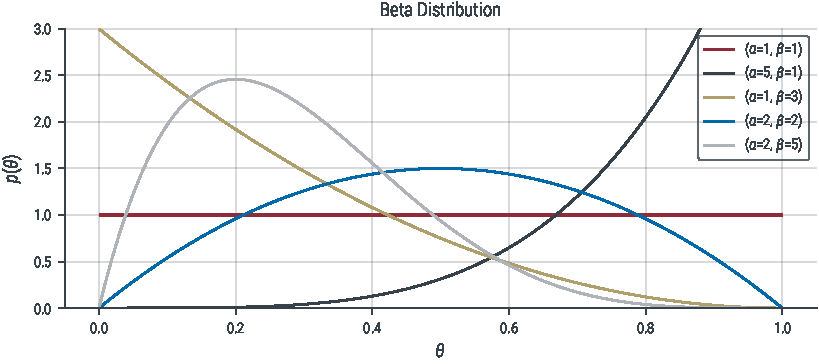
\includegraphics[scale = 0.75]{../figures/map/beta_distribution.pdf}}
        \end{figure}

        Notebook
    \end{frame}

    \begin{frame}{Coin Toss Problem with Prior}
        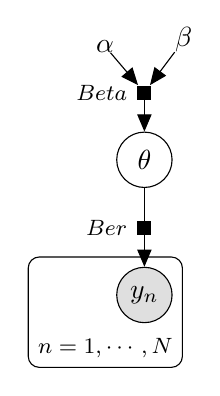
\begin{tikzpicture}
                
            \node[obs]                               (xn) {$y_n$};
            \node[latent, above=of xn] (mu) {$\mathbf{\theta}$};
            \factor[above=of xn] {y-f} {left:${Ber}$} {} {} ; %
            \node[const, above=1 of mu, xshift=0.5cm] (beta) {$\mathbf{\beta}$};
            \node[const, above=1 of mu, xshift=-0.5cm] (alpha) {$\mathbf{\alpha}$};
            \factor[above=of mu] {mu-f} {left:${Beta}$} {} {} ; %
            \plate{}{(xn)}{$n = 1, \cdots, N$};
            
            \edge {mu} {xn} ; %
            \edge {alpha,beta} {mu-f} ; %
            \edge  {mu-f}{mu} ; %
            
        \end{tikzpicture}
    \end{frame}

    \begin{frame}{Deriving $\theta_{MAP}$}
        \begin{itemize}
            \item \textbf{Recall}: $\theta_{\text{MAP}} = \arg \max_{\theta} \textcolor{myblue}{P(\theta|D)} = \arg \max_{\theta} \textcolor{mygreen}{P(D|\theta)} \cdot \textcolor{myred}{P(\theta)}$
            \pause
            \item The log-posterior for this coin-toss problem is given as,
            \pause
            \begin{equation*}
                \textcolor{myblue}{\log P (\theta | D)} = \sum_{i = 1}^{N} \textcolor{mygreen}{\log P (y_i | \theta)} + \textcolor{myred}{\log P (\theta)}
            \end{equation*}
            \pause 
            \begin{align*}
                \textcolor{myblue}{\log P (\theta | D)} = \sum_{i = 1}^{N} \textcolor{mygreen}{y_i \log \theta + (1 - y_i) \log (1 - \theta)} + \\ \textcolor{myred}{(\alpha - 1) \log \theta + (\beta - 1) \log (1 - \theta)}
            \end{align*}
        \end{itemize}
    \end{frame}

    \begin{frame}{Deriving $\theta_{MAP}$}
        \begin{equation*}
            \frac{\partial \log P (\theta | D)}{\partial \theta} = \frac{\sum_{i = 1}^{N} y_i}{\theta} - \frac{\sum_{i = 1}^{N} (1 - y_i)}{1 - \theta} + \frac{\alpha - 1}{\theta} - \frac{\beta - 1}{1 - \theta} = 0
        \end{equation*}

        \begin{equation*}
            \implies (1 - \theta) \sum_{i = 1}^{N} y_i + \theta \sum_{i = 1}^{N} (1 - y_i) + (1 - \theta) (\alpha - 1) - \theta (\beta - 1) = 0
        \end{equation*}

        \begin{equation*}
            \implies \sum_{i = 1}^{N} y_i - \theta \sum_{i = 1}^{N} y_i - N \theta + \theta \sum_{i = 1}^{N} y_i + \alpha - 1 - \theta \alpha  + \theta - \theta \beta + \theta = 0
        \end{equation*}

    \end{frame}

    \begin{frame}{Deriving $\theta_{MAP}$}

        \begin{equation*}
            \implies \sum_{i = 1}^{N} y_i + \alpha - 1 - \theta ( N + \alpha + \beta - 2) = 0
        \end{equation*}

        \begin{equation*}
            \implies \theta_{MAP} = \frac{\sum_{i = 1}^{N} y_i + \alpha - 1}{N + \alpha + \beta - 2}
        \end{equation*}
    \end{frame}

    \begin{frame}{Deriving $\theta_{MAP}$ (Coin toss context)}
        \begin{itemize} [<+->]
            \item Total number of tosses = $N$
            \item Number of heads ($y=1$) = $n_H$
            \item Number of tails ($y=0$)= $n_T$
            \item Pseudo heads  = $\alpha$
            \item Pseudo tails = $\beta$
            \item $\theta_{MAP} = \frac{n_H + \alpha - 1}{N + \alpha + \beta - 2}$
            \item Prior = Beta$(\alpha, \beta)$
            \item Posterior = Beta$(n_H + \alpha, n_T + \beta)$
        \end{itemize}
        
    \end{frame}

    \begin{frame}{Coin Toss Problem with Prior}
        \begin{figure}
            \centerline{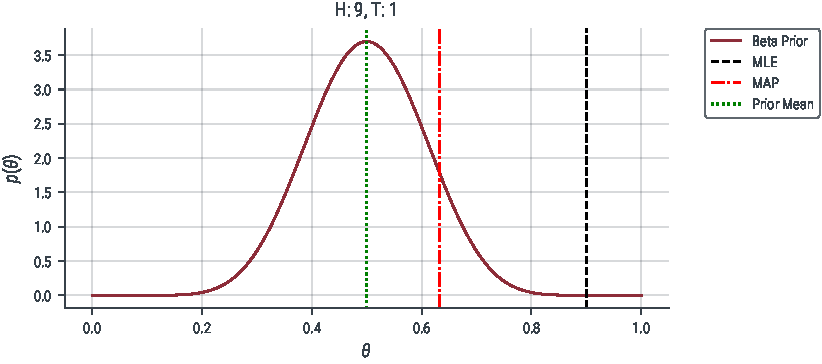
\includegraphics[scale = 0.75]{../figures/map/coin_toss_prior_mle_map.pdf}}
        \end{figure}

    Notebook
    \end{frame}
\end{section}


% \begin{section}{MAP for Coin Toss}
%     \begin{frame}{MLE for Coin Toss}
%         Assuming a coin with probability of heads $\theta$ (consider Bernoulli), the probability of observing $D = \{H, H, T, H, T, T, T, T\}$ is given by:
%         \begin{equation}
%             P(D|\theta) = \theta^3(1-\theta)^5
%         \end{equation}

%         \begin{equation}
%             \implies \hat{\theta}_{MLE} = \arg \max_{\theta} P(D|\theta) = 3/8 = 0.375
%         \end{equation}
%         However, we have prior knowledge that the coin is fair, i.e., $\theta = 0.5$. How do we incorporate this knowledge?
%     \end{frame}

%     \begin{frame}{MAP for Coin Toss}
%         \begin{itemize}
%             \item Bernoulli Likelihood: $P(D|\theta) = \theta^3(1-\theta)^5$
%             \item Beta Prior: $P(\theta) = \frac{\theta^{\alpha-1}(1-\theta)^{\beta-1}}{B(\alpha, \beta)}$
%             \item For a fair coin, take $\alpha = \beta = 10$
%             \item Solving for MAP gives, $\hat{\theta}_{MAP} = 0.46$
%             \item Closer to expected value of 0.5
%         \end{itemize}
%     \end{frame}

%     \begin{frame}{Pop Quiz}
%         \begin{enumerate}
%             \item Derive the expression for $\hat{\theta}_{MAP}$ of a Coin Toss for a Bernoulli likelihood and Beta prior.
            
%             Answer: $\hat{\theta}_{MAP} = \frac{n_H + (\alpha - 1)}{n_H + n_T + (\alpha - 1) + (\beta - 1)}$
%             \item How does the number of observations affect the MAP estimate?
%             \item Show that the posterior follows Beta$(n_H + \alpha, n_T + \beta)$. 
%         \end{enumerate}
%     \end{frame}
% \end{section}

    \begin{comment}
    \begin{frame}{MAP for Normal Distribution}
        To estimate MAP for Normal Distribution, we can have the following 3 cases:
        \begin{enumerate}
            \item unknown $\mu$, known $\sigma^2$
            \item known $\mu$, unknown $\sigma^2$
            \item unknown $\mu$, unknown $\sigma^2$
        \end{enumerate}
    \end{frame}


    \begin{frame}{unknown $\mu$, known $\sigma^2$}
        \begin{itemize}
            \item Consider a sequence of independent N observations, $D = \{ x_1, ... , x_N \}$ drawn from $\mathcal{N} (x_i | \mu, \sigma^2)$
            \pause
            \item Likelihood is given by (Note: only $\mu$ is a random variable, $\sigma^2$ is known and assumed fixed) $P (D | \mu, \sigma^2) = \mathcal{L} (\mu) = \prod_{i=1}^{N} \frac{1}{\sqrt{2 \pi \sigma^2}} \exp \left( - \frac{(x_i - \mu)^2}{2 \sigma^2} \right)$
            \pause
            \item Log-Likelihood is given by 
            $$
            \log P (D | \mu, \sigma^2) = \mathcal{LL} (\mu) = \sum_{i=1}^{N} \left( - \frac{1}{2} \log (2 \pi \sigma^2) - \frac{(x_i - \mu)^2}{2 \sigma^2} \right)
            $$
            
            $$
            \implies \mathcal{LL} (\mu) = - \frac{N}{2} \log (2 \pi \sigma^2) - \frac{1}{2 \sigma^2} \sum_{i=1}^{N} (x_i - \mu)^2
            $$
        \end{itemize}
    \end{frame}

    \begin{frame}{Obtaining $\mu_{MLE}$}
        \begin{itemize}
            \item For MLE for $\mu$, we set
            $$
            \frac{\partial \mathcal{LL} (\mu)}{\partial \mu} = 0 - \left( - \frac{1}{2 \sigma^2} \sum_{i = 1}^{N} 2 (x_i - \mu) \right) = \frac{1}{\sigma^2} (\sum_{i = 1}^{N} x_i - N \mu) = 0
            $$
            or
            $$
            \mu_{MLE} = \frac{\sum_{i = 1}^{N} x_i}{N} 
            $$
            \pause
            \item However, similar to Coin Toss problem, this is prone to overfit.
        \end{itemize}
    \end{frame}

    \begin{frame}{Incorporating Prior Information}
        \begin{itemize}
            \item Since we need a prior over $\mu$, we can choose $P (\mu | \mu_0, \sigma_0^2) = \mathcal{N} (\mu | \mu_0, \sigma_0^2)$
            \pause
            \item The Posterior for $\mu$ is given by
            $$
            P (\mu | D) \propto P (D | \mu) P (\mu) \propto \prod_{i = 1}^{N} \exp \left( - \frac{(x_i - \mu)^2}{2 \sigma^2} \right) \exp \left( - \frac{(\mu - \mu_0)^2}{2 \sigma_0^2} \right)
            $$
            \pause
            \item Simplifying, we get
            $$
            P (\mu | D) \propto \exp \left( - \frac{(\mu - \mu_N)^2}{2 \sigma_N^2} \right)
            $$
            where,
            $$
            (\mu_N, \sigma_N) = \left(\frac{\frac{\sigma^2}{N}}{\sigma_0 + \frac{\sigma^2}{N}} + \frac{\sigma_0^2}{\sigma_0 + \frac{\sigma^2}{N}} \frac{\sum_{i = 1}^{N} x_i}{N}, \left( \frac{1}{\sigma_0^2} + \frac{N}{\sigma^2} \right)^{-1} \right)
            $$
        \end{itemize}
    \end{frame}

    \begin{frame}{Obtaining MAP}
        \begin{itemize}
            \item For MAP, we set
            $$
            \frac{\partial \log P (\mu | D)}{\partial \mu} = - \frac{1}{2 \sigma^2} \sum_{i = 1}^{N} -2 (x_i - \mu) - \frac{1}{2 \sigma_0^2} \sum_{i = 1}^{N} 2 (\mu - \mu_0) = 0
            $$
            \pause
            \begin{align*}
                \implies \frac{1}{\sigma^2} (\sum_{i = 1}^{N} x_i - N \mu) - \frac{N}{\sigma_0^2} (\mu - \mu_0) = \\ \mu \left( - \frac{N}{\sigma^2} - \frac{N}{\sigma_0^2} \right) + \frac{\sum_{i = 1}^{N} x_i}{\sigma^2} + \frac{N \mu_0}{\sigma_0^2} = 0                
            \end{align*}
            \pause
            $$
            \mu_{MAP} = \frac{\frac{\mu_0}{\sigma_0^2} + \frac{\frac{\sum_{i = 1}^{N} x_i}{N}}{\sigma^2}}{\frac{1}{\sigma_0^2} + \frac{1}{\sigma^2}} = \frac{\sigma^2 \mu_0 + \sigma_0^2 \frac{\sum_{i = 1}^{N} x_i}{N}}{\sigma_0^2 + \sigma^2}
            $$
        \end{itemize}
    \end{frame}

    \begin{frame}{known $\mu$, unknown $\sigma^2$}
        Assuuming $\mu$ is known, the conjugate prior for $\sigma^2$ is Inverse Gamma$(\alpha_0, \beta_0)$ which gives,
        \begin{equation*}
            P(\sigma^2|\alpha_0, \beta_0) \propto \frac{1}{(\sigma^2)^{\alpha_0 + 1}} \exp\left(-\frac{\beta_0}{\sigma^2}\right)
        \end{equation*}

        $\therefore$ The posterior is given by,
        \begin{equation*}
            P(\sigma^2|D; \alpha_0, \beta_0) \sim \text{Inverse Gamma} \left( \alpha_0 + \frac{n}{2}, \beta_0 + \frac{\sum_{i=1}^n (x_i-\mu)}{2} \right)
        \end{equation*}
    \end{frame}

    \begin{frame}{unknown $\mu$, unknown $\sigma^2$}
        Assuuming both $\mu$ and $\sigma^2$ are unknown, the conjugate prior for $\mu$ and $\sigma^2$ (or Precision $\tau = \frac{1}{\sigma^2}$) is as follows,
        \begin{align*}
            D | \mu, \tau &\sim \mathcal{N}(\mu, \tau^{-1}) \\
            \mu | \tau &\sim \mathcal{N}(\mu_0, (\kappa_0\tau)^{-1}) \\
            \tau &\sim \text{Gamma}(\alpha_0, \beta_0)
        \end{align*}

        $\therefore$ The posterior is given by,
        \begin{align*}
            \mu | D, \tau &\sim \mathcal{N} \left( \frac{\kappa_0\mu_0 + n\bar{x}}{\kappa_0 + n}, \left( \kappa_0 + n \right)^{-1} \right) \\
            \tau | D &\sim \text{Gamma} \left( \alpha_0 + \frac{n}{2}, \beta_0 + \frac{1}{2}\sum_{i=1}^n (x_i-\mu)^2 + \frac{\kappa_0n(\bar{x}-\mu_0)^2}{2(\kappa_0 + n)} \right)
        \end{align*}
    \end{frame}
\end{section}

\begin{section}{MAP for Linear Regression}
    \begin{frame}{MLE for Linear Regression}
        \begin{itemize}
            \item Consider a dataset $D = \{ (x_1, y_1) ... (x_N, y_N) \}$ where $x_i \in \mathbb{R}^d$ and $y_i \in \mathbb{R}$.
            \pause
            \item Suppose the data is generated from a linear model with additive Gaussian noise, i.e., $y_i = \theta^T x_i + \epsilon_i$ where $\epsilon_i \sim \mathcal{N}(0, \sigma^2)$.
        \end{itemize}
        \pause
        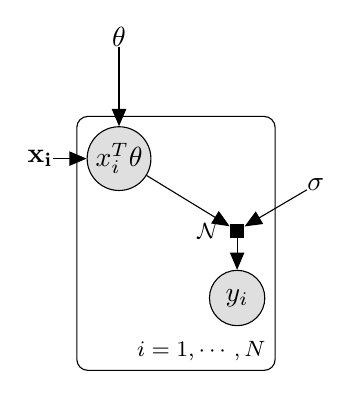
\begin{tikzpicture}   
            \node[obs]                               (xit) {$x_i^T\theta$};
            \node[obs, below=1 of xit, xshift = 1.5cm] (yi) {$y_i$};
            \node[const, xshift=-1cm](xi) {$\mathbf{x_i}$};
            \node[const, above=1 of xit](theta)
            {$\mathbf{\theta}$};

            \factor[above=of yi] {y-f} {left:${\mathcal{N}}$} {} {} ; %
            \node[const, above=1 of yi, xshift=1cm] (sigma) {$\mathbf{\sigma}$};
            \plate{}{(xit)(yi)}{$i = 1, \cdots, N$};
            \edge{theta}{xit}
            \edge{xit}{y-f}
            \edge{sigma}{y-f}
            \edge{xi}{xit}
            \edge{y-f}{yi}     
        \end{tikzpicture}
    \end{frame}
\end{comment}
    \begin{frame}{MLE for Linear Regression}
        \begin{itemize}
            \item Consider a dataset $D = \{ (x_1, y_1) ... (x_N, y_N) \}$ where $x_i \in \mathbb{R}^d$ and $y_i \in \mathbb{R}$.
            \item Suppose the data is generated from a linear model with additive Gaussian noise, i.e., $y_i = \theta^T x_i + \epsilon_i$ where $\epsilon_i \sim \mathcal{N}(0, \sigma^2)$.
        \end{itemize}
        \begin{figure}
            \centerline{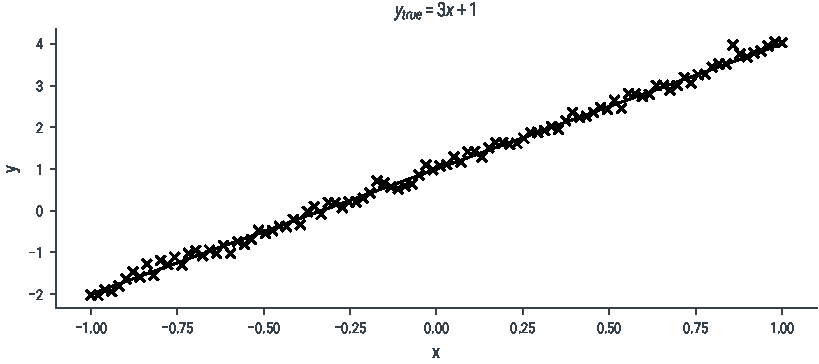
\includegraphics[scale = 0.75]{../figures/map/linreg_data.pdf}}
        \end{figure}
        
    \end{frame}

    \begin{frame}{MLE for Linear Regression}
        \begin{itemize}
            \item The likelihood is given by,
            $P(y_i | x_i, \theta) = \mathcal{N}(y_i | \theta^T x_i, \sigma^2)$
            \item \textbf{Recall}: The negative log-likelihood is given by,
            $\mathcal{NLL}(\theta) = \frac{1}{2 \sigma^2} \left( y - X \theta \right)^T \left( y - X \theta \right)$
            \item \textbf{Recall}: The MLE is given by,
            $\theta_{MLE} =  \arg \min_{\theta} \mathcal{NLL} (\theta) = \left( X^T X \right)^{-1} X^T y$
        \end{itemize}
        \begin{figure}
            \centerline{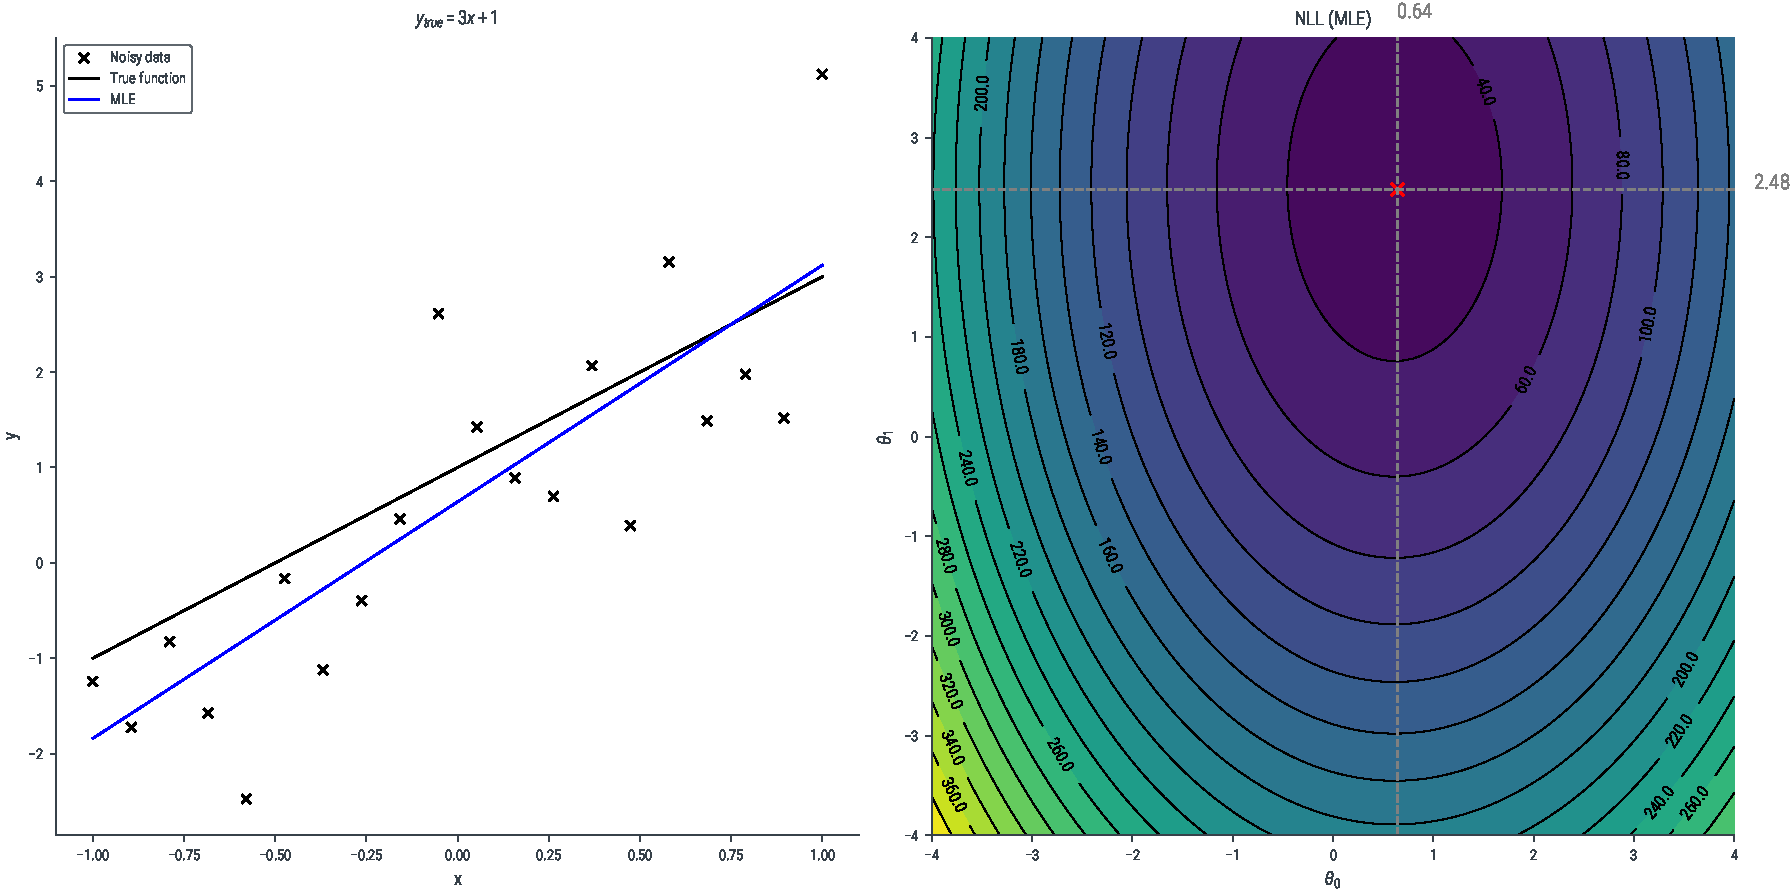
\includegraphics[scale = 0.35]{../figures/map/linreg_mle.pdf}}
        \end{figure}

    \end{frame}

  

    \begin{frame}{MAP for Linear Regression}
        %Considering a zero-mean Gaussian prior on the weights, i.e., $P(\theta) = \mathcal{N}(\theta|\mathbf{0}, \sigma_0^2)$, we have

        %$\textcolor{myblue}{P (\theta | D)} \propto \textcolor{mygreen}{P (D | \theta)} \textcolor{myred}{P (\theta)}$

        %$\theta_{MAP} = \arg \min \textcolor{myblue}{\log P (\theta | D)} = \arg \min \textcolor{mygreen}{\mathcal{NLL} (\theta)} + \textcolor{myred}{\log P (\theta)}$

        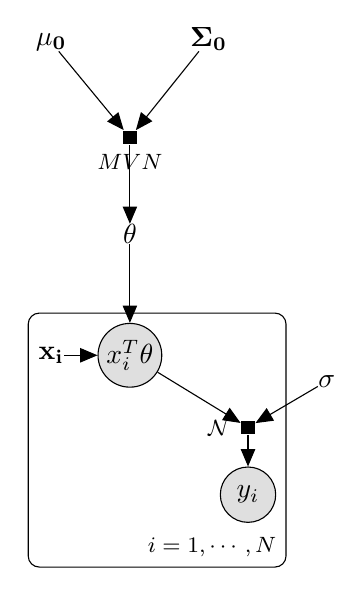
\begin{tikzpicture}   
            \node[obs]                               (xit) {$x_i^T\theta$};
            \node[obs, below=1 of xit, xshift = 1.5cm] (yi) {$y_i$};
            \node[const, xshift=-1cm](xi) {$\mathbf{x_i}$};
            \node[const, above=1 of xit](theta)
            {$\mathbf{\theta}$};
            
            \factor[above=1 of theta] {theta-f} {below:${{MVN}}$} {} {} ; %
            \edge{theta-f}{theta}
            \node[const, above=1 of theta-f, xshift=1cm](sigma) {$\mathbf{\Sigma_0}$};
            \node[const, above=1 of theta-f, xshift=-1cm](mu) {$\mathbf{\mu_0}$};
            \edge{sigma}{theta-f}
            \edge{mu}{theta-f}

            \factor[above=of yi] {y-f} {left:${\mathcal{N}}$} {} {} ; %
            \node[const, above=1 of yi, xshift=1cm] (sigma) {$\mathbf{\sigma}$};
            \plate{}{(xi)(xit)(yi)}{$i = 1, \cdots, N$};
            \edge{theta}{xit}
            \edge{xit}{y-f}
            \edge{sigma}{y-f}
            \edge{xi}{xit}
            \edge{y-f}{yi}     
        \end{tikzpicture}

    \end{frame}

    \begin{frame}{MAP for Linear Regression}
        As per Bayes' rule,
        $$
        P (\theta | D) = \frac{P (D | \theta) P (\theta)}{P (D)}
        $$

        \pause

        \begin{itemize}
            \item Log-Likelihood: $\mathcal{LL} (\theta) = \log P (D | \theta) = \log \prod_{i = 1}^{N} \mathcal{N}(y_i | x_i^T \theta, \sigma^2)$
            \item Prior: $P (\theta) = \mathcal{N}(\theta | \mu_0, \Sigma_0)$
            \item Log-Prior: $\log P (\theta) = \log \mathcal{N}(\theta | \mu_0, \Sigma_0)$
            \item Log-Joint: $\log P (\theta | D) = \log P (D | \theta) + \log P (\theta)$
        \end{itemize}
    \end{frame}

    \begin{frame}{MAP for Linear Regression}
        Notebook
    \end{frame}
        
    \begin{frame}{MAP for Linear Regression}
        \begin{equation*}
            \theta_{MAP} = \arg \min \textcolor{myblue}{\log P (\theta | D)} = \arg \min \textcolor{mygreen}{\mathcal{NLL} (\theta)} + \textcolor{myred}{\log P (\theta)}
        \end{equation*}
    \end{frame}
    

    \begin{frame}{Using zero-mean Gaussian prior}
        $P(\theta) = MVN(\mu_0, \Sigma_0)$
    
        \pause  Assume: $\mu_0 = \vec{0}$, $\Sigma_0 = \sigma_0^2 \mathbf{I}$
        \pause \begin{equation*}
            \theta_{MAP} = \arg \min \textcolor{myblue}{\log P (\theta | D)} = \arg \min \textcolor{mygreen}{\mathcal{NLL} (\theta)} + \textcolor{myred}{\log P (\theta)}
        \end{equation*}
        \pause
        We get
        \begin{equation*}
            \theta_{MAP} = \arg \min \textcolor{mygreen}{\frac{1}{2 \sigma^2} (y - X\theta)^T (y - X\theta)} + \textcolor{myred}{\frac{1}{\sigma_0^2} \theta^T \theta}
        \end{equation*}
        \pause    
        \begin{tcolorbox}[colback=metropolisblue!5,colframe=metropolisblue,title=Question]
            What does this expression remind you of?
        \end{tcolorbox}
        \pause
        Answer: \textcolor{red}{Ridge Regression}
    \end{frame}

    \begin{frame}{Using zero-mean Laplace}
        Assume: each $\theta_i \sim Laplace(0, \sigma_0)$
        \pause \begin{equation*}
            \theta_{MAP} = \arg \min \textcolor{myblue}{\log P (\theta | D)} = \arg \min \textcolor{mygreen}{\mathcal{NLL} (\theta)} + \textcolor{myred}{\log P (\theta)}
        \end{equation*}
        \pause
        We get
        \begin{equation*}
            \theta_{MAP} = \arg \min \textcolor{mygreen}{\frac{1}{2 \sigma^2} (y - X\theta)^T (y - X\theta)} + \lambda\textcolor{myred}{|\theta|}
        \end{equation*}
        \pause    
        \begin{tcolorbox}[colback=metropolisblue!5,colframe=metropolisblue,title=Question]
            What does this expression remind you of?
        \end{tcolorbox}
        \pause
        Answer: \textcolor{red}{LASSO Regression}
    \end{frame}


    \begin{comment}
        
  
    \begin{frame}{Using zero-mean Gaussian prior}
        \begin{figure}
            \centerline{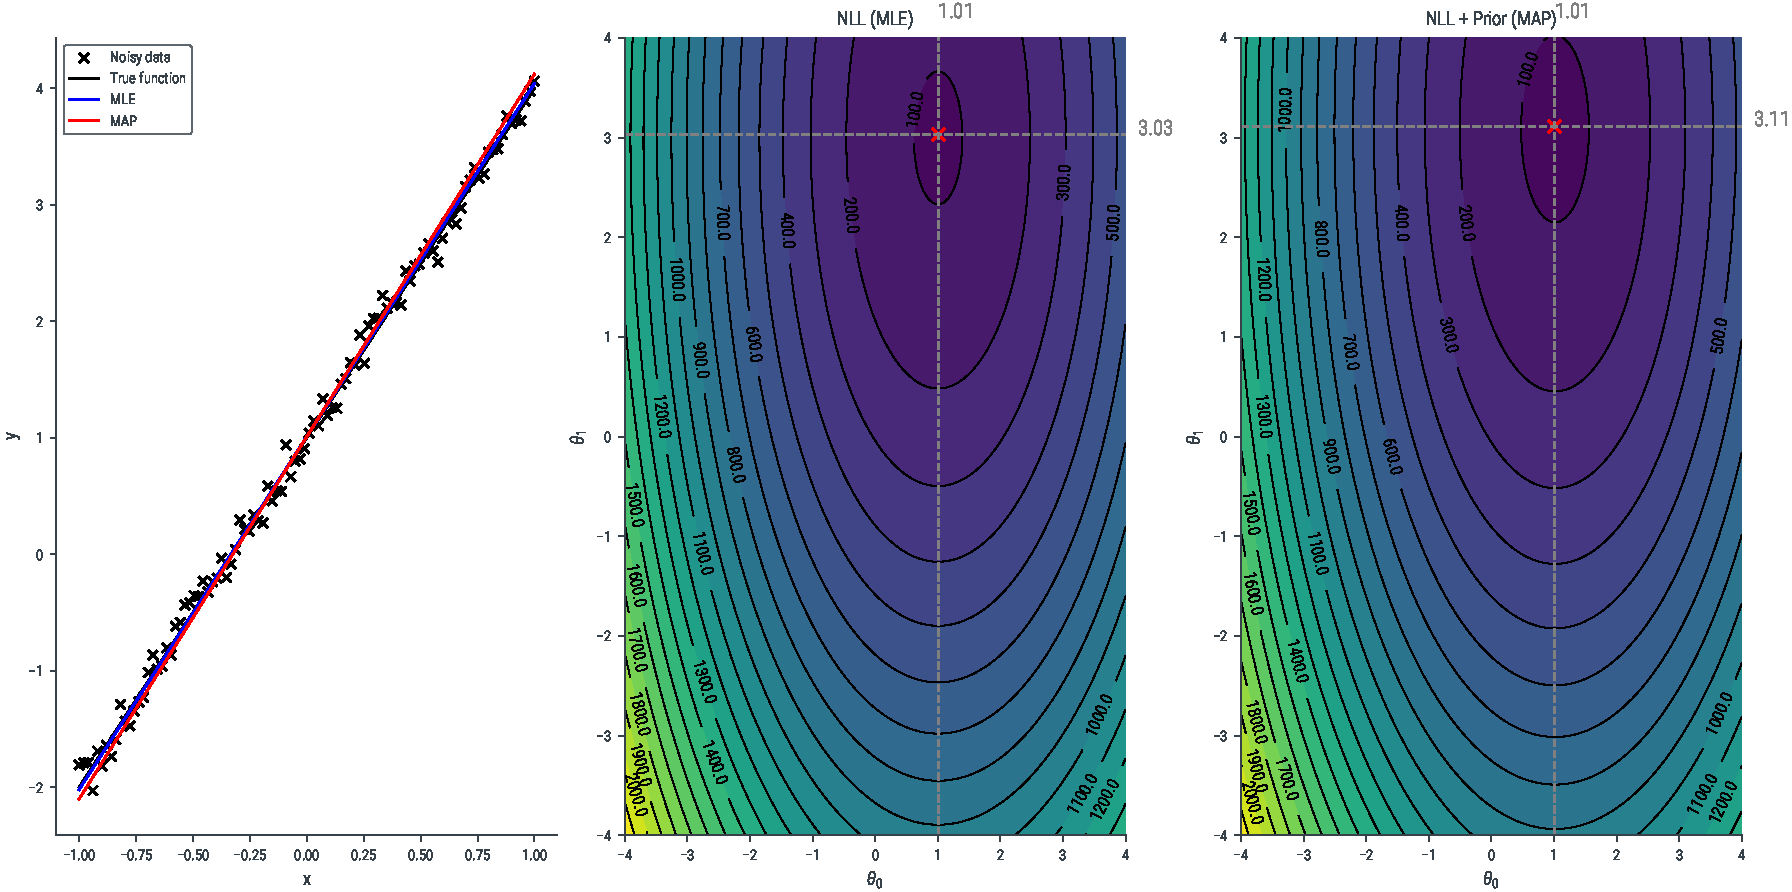
\includegraphics[scale = 0.40]{../figures/map/linreg_mle_map.pdf}}
        \end{figure}
        Notebook
    \end{frame}
\end{comment}

    \begin{frame}{Using Laplace prior}
        We can also use a Laplace prior on the weights, i.e., 
        $$P(\theta) = \frac{1}{2b_0} \exp \left( - \frac{| x - \mu |}{b_0} \right)$$

        \vspace{10pt}
        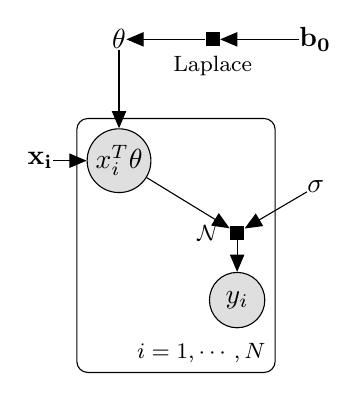
\begin{tikzpicture}   
            \node[obs]                               (xit) {$x_i^T\theta$};
            \node[obs, below=1 of xit, xshift = 1.5cm] (yi) {$y_i$};
            \node[const, xshift=-1cm](xi) {$\mathbf{x_i}$};
            \node[const, above=1 of xit](theta)
            {$\mathbf{\theta}$};
            
            \factor[right=1 of theta] {theta-f} {below:${\text{Laplace}}$} {} {} ; %
            \edge{theta-f}{theta}
            \node[const, right=1 of theta-f](b) {$\mathbf{b_0}$};
            \edge{b}{theta-f}

            \factor[above=of yi] {y-f} {left:${\mathcal{N}}$} {} {} ; %
            \node[const, above=1 of yi, xshift=1cm] (sigma) {$\mathbf{\sigma}$};
            \plate{}{(xit)(yi)}{$i = 1, \cdots, N$};
            \edge{theta}{xit}
            \edge{xit}{y-f}
            \edge{sigma}{y-f}
            \edge{xi}{xit}
            \edge{y-f}{yi}     
        \end{tikzpicture}
    \end{frame}

    \begin{frame}{Using Laplace prior}
        The MAP takes the form,
        \begin{equation*}
            \theta_{MAP} = \arg \min \textcolor{mygreen}{\frac{1}{2 \sigma^2} (y - X\theta)^T (y - X\theta)} + \textcolor{myred}{\frac{1}{b_0} |\theta_i|}
        \end{equation*}
        \pause
        \begin{tcolorbox}[colback=metropolisblue!5,colframe=metropolisblue,title=Question]
            What does this expression remind you of?
        \end{tcolorbox}
        \pause
        Answer: \textcolor{red}{Lasso Regression}
    \end{frame}

    \begin{frame}{Using Laplace prior}
        \begin{figure}
            \centerline{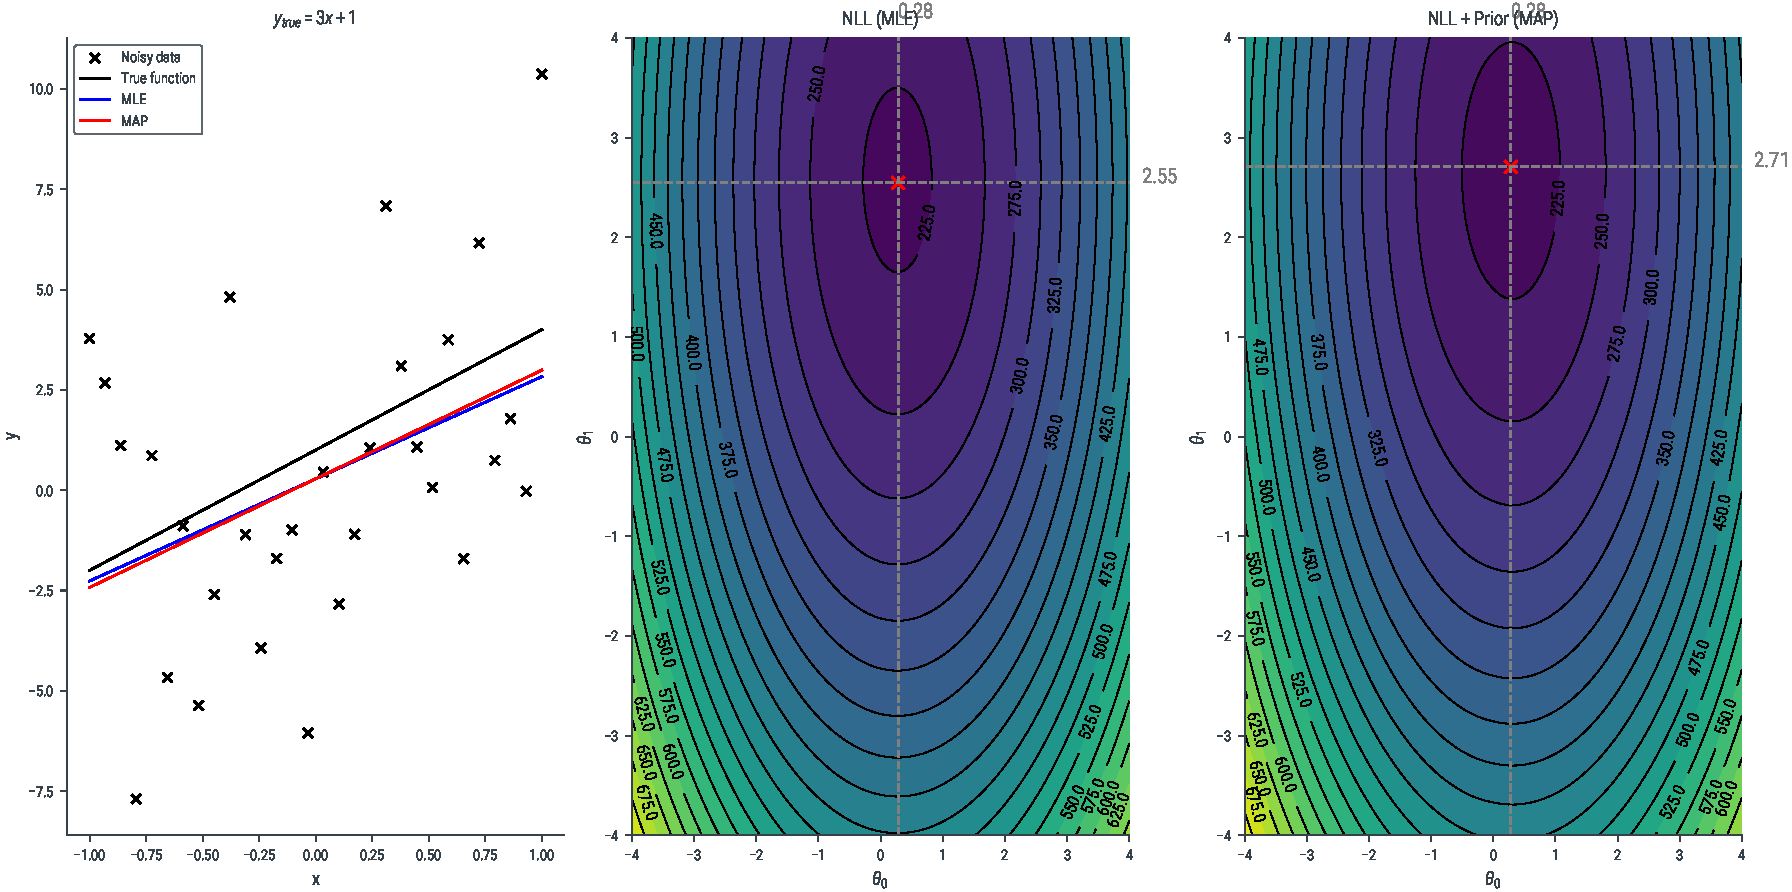
\includegraphics[scale = 0.40]{../figures/map/linreg_mle_map_laplace.pdf}}
        \end{figure}
        Notebook
    \end{frame}

\begin{section}{MAP for Logistic Regression}
    \begin{frame}{MLE for Logistic Regression}
        Consider a dataset $D = \{ (x_1, y_1) ... (x_N, y_N) \}$, where $x_i \in \mathbb{R}^d$ and $y_i \in \{ 0, 1 \}$ such that
        $$ P(y = 1 | x) = \hat{y} = \frac{1}{1 + \exp (- X^T \theta)} = \sigma (X^T \theta)$$
        Take $y \sim \text{Bernoulli} \left( \sigma (X^T \theta) \right)$

        \pause
        The likelihood is given by
        $$ \mathcal{L} (\theta) = \prod_{i=1}^{N} \hat{y_i}^{y_i} (i - \hat{y_i})^{1 - y_i}$$ 
        $$ \implies \mathcal{LL} (\theta) = \sum_{i=1}^{N} y_i \log \hat{y_i} + (1 - y_i) \log (1 - \hat{y_i}) $$ 
    \end{frame}

    \begin{frame}{MLE for Logistic Regression}
        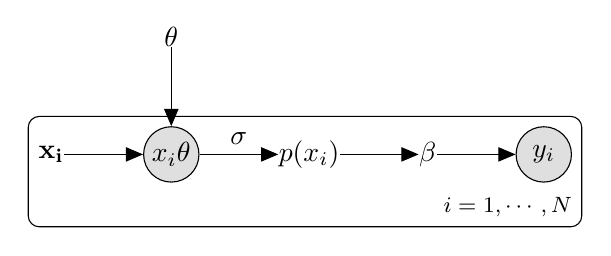
\begin{tikzpicture}

            \node[obs] (x_i_theta) {$x_i\theta$};
            \node[const, left=of x_i_theta] (xi) {$\mathbf{x_i}$};
            \node[const, above=of x_i_theta] (theta) {$\mathbf{\theta}$};
            \node[const, right=of x_i_theta] (pxi) {$p(x_i)$};
            \node[const, right=of pxi] (beta) {$\beta$};
            \node[obs, right=of beta] (yi_out) {$y_i$};
            \plate {plate1} {(xi)(x_i_theta)(yi_out)} {$i = 1, \cdots, N$};
            
            \draw[->] (xi) -- (x_i_theta);
            \draw[->] (theta) -- (x_i_theta);
            \draw[->] (x_i_theta) -- node[above] {$\sigma$} (pxi); % Adding "sigma" text
            \draw[->] (pxi) -- (beta);
            \draw[->] (beta) -- (yi_out);
            
        \end{tikzpicture}

        Binary Classification:
        $$
            P (Y = 1 | X) = \frac{1}{1 + e^{- (\theta_0 + \theta_1 X)}}
        $$

        $$
            \therefore \mathcal{LL} (\theta) = \sum_{i=1}^{N} y_i \log p(x_i) + (1 - y_i) \log (1 - p(x_i))
        $$
    \end{frame}

    \begin{frame}{Using zero-mean Gaussian prior}
        Considering a zero-mean Gaussian prior on the weights, i.e., $P(\theta) = \mathcal{N}(\theta|0, \sigma_0^{2})$, the MAP is given by,
        \begin{equation*}
            \theta_{MAP} = \arg \min \log(1 + \exp(- \theta^T X)) + \frac{1}{\sigma_0^2} \theta^T \theta
        \end{equation*}
        
    \end{frame}

    \begin{frame}{Using Laplace prior}
        Considering a Laplace prior on the weights, i.e., $P(\theta) = \prod_{D} \text{Laplace} (\theta_i|0, b_0) \propto \prod_{D} \exp(- \frac{1}{b_0} |\theta_i|)$
        , the MAP is given by,
        \begin{equation*}
            \theta_{MAP} = \arg \min  \log(1 + \exp(- \theta^T X)) + \frac{1}{b_0} |\theta|
        \end{equation*}
        
    \end{frame}

    \begin{frame}{MAP for Logistic Regression}
        Self-Study: Modify the code for Linear Regression to implement MAP for Logistic Regression.
    \end{frame}
    
\end{section}

\end{document}